\chapter{Condotto con Bump}
\label{cap:bump}

\section{Descrizione del Caso Studio}

Il primo caso studio analizzato riguarda un \textbf{condotto piano con un rialzo gaussiano
(\textit{bump}) sul fondo}. Fisicamente il dominio rappresenta la metà inferiore di un condotto
convergente-divergente, sfruttando la simmetria del problema rispetto all'asse orizzontale.

Il dominio è un rettangolo di dimensioni $L \times h = 1 \times 0.3$ sul quale la parete
inferiore presenta un ostacolo di forma spline con apice di altezza $h/10 = 0.03$ nella
sezione centrale. Le coordinate caratteristiche sono:
\begin{itemize}
  \item Vertice sinistro inferiore: $(0, 0)$ -- bordo di \textbf{Inlet}
  \item Vertice destro inferiore: $(1, 0)$ -- bordo di \textbf{Outlet}
  \item Tetto del dominio: $y = 0.3$
  \item Apice del bump: $(0.5,\, 0.03)$
  \item Piede sinistro del bump: $(0.375,\, 0)$
  \item Piede destro del bump: $(0.625,\, 0)$
\end{itemize}

Il flusso attraversa il condotto da sinistra verso destra con numero di Mach subsonico
$M_{\rm in} = 0.3$. In assenza di onde d'urto e con equazioni di Eulero, il campo di entropia
dovrebbe essere identicamente nullo; la deviazione da tale valore fornisce quindi una misura
diretta dell'errore numerico.

\begin{figure}[H]
  \centering
  \begin{tikzpicture}[scale=5.0, >=Stealth]
    % Pareti esterne
    \draw[thick] (0,0.3) -- (1,0.3);   % tetto
    \draw[thick,blue!70!black,->] (-0.05,0.1) -- (0,0.1) node[right,black,xshift=2pt]{};
    % Inlet
    \draw[very thick, green!60!black] (0,0) -- (0,0.3) node[midway,left]{Inlet};
    % Outlet
    \draw[very thick, red!70!black] (1,0) -- (1,0.3) node[midway,right]{Outlet};
    % Wall (tetto)
    \draw[very thick, gray] (0,0.3) -- (1,0.3) node[midway, above]{Wall};
    % Bump: spline approssimata con curve di Bezier
    \draw[very thick, gray]
      (0,0) -- (0.375,0) .. controls (0.42,0) and (0.45,0.03) ..
      (0.5,0.03) .. controls (0.55,0.03) and (0.58,0) .. (0.625,0) -- (1,0);
    \node[below] at (0.5,-0.01) {\small Parete (bump)};
    % Dimensioni
    \draw[<->,gray!60] (0,-0.04) -- (1,-0.04) node[midway,below]{\small $L = 1$};
    \draw[<->,gray!60] (1.04,0) -- (1.04,0.3) node[midway,right]{\small $h = 0.3$};
    \draw[<->,gray!60] (0.5,0) -- (0.5,0.03) node[midway,right]{\small $h/10$};
    % Freccia flusso
    \foreach \y in {0.08, 0.15, 0.22}
      \draw[->, blue!60, thick] (-0.07,\y) -- (0,\y);
    \node[left, blue!60] at (-0.07,0.15) {\small $M_{\rm in}=0.3$};
  \end{tikzpicture}
  \caption{Schema del dominio computazionale per il caso bump (non in scala).}
  \label{fig:dominio_bump}
\end{figure}

\section{Condizioni di Inlet e Outlet}

\begin{table}[h!]
\centering
\begin{tabular}{|l|l|l|}
\hline
 & \textbf{Inlet} & \textbf{Outlet} \\ \hline
\textbf{$T^\circ$} & 1 & - \\ \hline
\textbf{$p^\circ$} & 1 & - \\ \hline
\textbf{p} & - & 0.9395 \\ \hline
\textbf{M} & 0.3 & - \\ \hline
\textbf{Alpha} & 0 & - \\ \hline
\end{tabular}
\caption{Condizioni di Inlet e Outlet - Canale con Bump}
\label{tab:bump_conditions}
\end{table}

\section{Generazione della Mesh -- File \texttt{bump.geo}}
\label{sec:bump_geo}

\subsection{Struttura Generale del File}

Il file \texttt{bump.geo} definisce la geometria e produce una \textbf{mesh strutturata a
quadrilateri}. Si riporta il file commentato in dettaglio:

\begin{lstlisting}[style=gmsh, caption={File \texttt{bump.geo} -- geometria e mesh strutturata.}, label={lst:bump_geo}]
Mesh.MshFileVersion = 2.2;

// --- Parametri globali del dominio ---
L  = 1;    // lunghezza del dominio lungo x
h  = 0.3;  // altezza del dominio lungo y
lc = 0.05; // lunghezza caratteristica di default

// --- Quattro angoli del rettangolo ---
Point(1) = {0,   0,   0, lc}; // angolo inferiore sinistro (Inlet-Parete)
Point(2) = {L,   0,   0, lc}; // angolo inferiore destro  (Outlet-Parete)
Point(3) = {L,   h,   0, lc}; // angolo superiore destro  (Outlet-Tetto)
Point(4) = {0,   h,   0, lc}; // angolo superiore sinistro(Inlet-Tetto)

// --- Punti del bump ---
Point(5) = {L/2,      h/10, 0, lc}; // apice (massima altezza)
Point(6) = {L/2-L/8,  0,    0, lc}; // piede sinistro (0.375, 0)
Point(7) = {L/2+L/8,  0,    0, lc}; // piede destro   (0.625, 0)

// --- Linee del contorno esterno (esclusa la parete con bump) ---
Line(1) = {2, 3}; // bordo destro (Outlet)
Line(2) = {3, 4}; // tetto
Line(3) = {4, 1}; // bordo sinistro (Inlet)

// --- Spline per la parete inferiore con bump ---
// Si includono TUTTI i punti: angoli + piedi bump + apice
// L'ordine definisce il verso di percorrenza (da 1 a 2)
Spline(4) = {1, 6, 5, 7, 2};

// --- Chiusura del contorno ---
// Le linee devono formare un loop orientato in senso antiorario
Line Loop(1) = {1, 2, 3, 4};

// --- Superficie del dominio ---
Plane Surface(1) = {1};
\end{lstlisting}

\subsection{Definizione della Mesh Strutturata}
\label{sec:bump_transfinite}

La parte più significativa del file riguarda la generazione della griglia strutturata tramite
i comandi \texttt{Transfinite}:

\begin{lstlisting}[style=gmsh, caption={Comandi Transfinite per la mesh strutturata del bump.}, label={lst:bump_transfinite}]
// -- Linea 1: Outlet (verticale destra) --
// 30 nodi, crescita geometrica con ragione 1.1 dal basso verso l'alto
// (verso aumentante: dal punto 2 al punto 3)
Transfinite Line {1} = 30 Using Progression 1.1;

// -- Linea 3: Inlet (verticale sinistra) --
// 30 nodi, ma con tag NEGATIVO (-3): la progressione geometrica
// parte dal punto 1 (in basso), cioe' lo stesso verso della linea 1
// Il segno negativo inverte il verso di percorrenza della linea (4->1)
Transfinite Line {-3} = 30 Using Progression 1.1;

// -- Linea 2: Tetto (orizzontale superiore) --
// 60 nodi con distribuzione BUMP centrata:
// la mesh e' piu' fitta al centro del tetto (sopra il bump)
// e si dirada verso i due estremi
Transfinite Line {2} = 60 Using Bump 3;

// -- Linea 4: Parete inferiore con bump --
// 60 nodi con distribuzione BUMP centrata:
// addensamento nella zona del bump dove si hanno i gradienti maggiori
// Il parametro 3 controlla il rapporto tra elemento centrale ed estremi
Transfinite Line {4} = 60 Using Bump 3;

// Definizione della superficie strutturata:
// si elencano i quattro punti ANGOLO della superficie
Transfinite Surface {1} = {1, 2, 3, 4};

// Conversione da triangoli a quadrilateri (mesh a quadrilateri puri)
Recombine Surface{1};

// --- Tag per le condizioni al contorno ---
Physical Surface(1) = {1};   // DOMINIO DI CALCOLO (tag 1)
Physical Line(99)   = {4, 2}; // PARETE SOLIDA (tag 99): bump + tetto
Physical Line(2)    = {3};    // INLET (tag 2): bordo sinistro
Physical Line(3)    = {1};    // OUTLET (tag 3): bordo destro
\end{lstlisting}

\paragraph{Commento sulle scelte di raffinamento.}
La distribuzione \texttt{Bump} sulle linee orizzontali (linee 2 e 4) è motivata fisicamente:
il bump genera un accelerazione del flusso nella sezione di gola (convergente) e una
decelerazione nel tratto divergente. I gradienti più intensi di velocità e pressione si
trovano in prossimità del punto di massima curvatura del bump, ovvero nella zona centrale,
giustificando l'addensamento simmetrico.

La distribuzione \texttt{Progression} sulle linee verticali (linee 1 e 3) addensa le celle
nella parte bassa del condotto, vicino alla parete, dove si sviluppano gli strati limite.
Il segno negativo su \texttt{-3} assicura che la progressione cresca nella stessa direzione
su entrambi i lati (dal basso verso l'alto), mantenendo la coerenza topologica richiesta
da \texttt{Transfinite Surface}.

\begin{figure}[H]
  \centering
  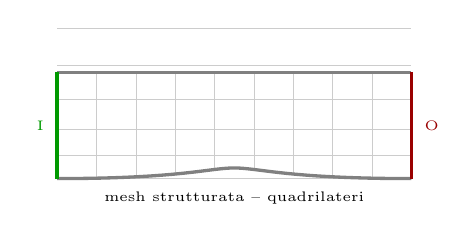
\begin{tikzpicture}[scale=4.5]
    % Visualizzazione schematica della mesh strutturata
    % Nodi verticali con progressione
    \foreach \i in {0,1,...,5} {
      \pgfmathsetmacro{\xL}{0.0}
      \pgfmathsetmacro{\xR}{1.0}
      \pgfmathsetmacro{\y}{\i*0.3/5 + 0.005*\i*\i}
      \draw[gray!40, very thin] (\xL,\y) -- (\xR,\y);
    }
    % Nodi orizzontali con bump
    \foreach \j in {0,1,...,9} {
      \pgfmathsetmacro{\x}{\j/9}
      % calcolo altezza bump
      \pgfmathsetmacro{\bh}{0.03*exp(-25*(\x-0.5)*(\x-0.5))}
      \draw[gray!40, very thin] (\x,\bh) -- (\x,0.3);
    }
    % Parete con bump
    \draw[very thick, gray] (0,0) .. controls (0.35,0) and (0.43,0.03) ..
      (0.5,0.03) .. controls (0.57,0.03) and (0.65,0) .. (1,0);
    % Tetto
    \draw[very thick, gray] (0,0.3) -- (1,0.3);
    % Inlet/Outlet
    \draw[very thick, green!60!black] (0,0) -- (0,0.3);
    \draw[very thick, red!60!black] (1,0) -- (1,0.3);
    % Label
    \node[below, font=\tiny] at (0.5,-0.01) {mesh strutturata -- quadrilateri};
    \node[left, font=\tiny, green!60!black] at (-0.01,0.15) {I};
    \node[right, font=\tiny, red!60!black] at (1.01,0.15) {O};
  \end{tikzpicture}
  \caption{Schema della mesh strutturata per il caso bump (30$\times$60 nodi, quadrilateri).}
  \label{fig:mesh_strutturata_bump}
\end{figure}

\section{Mesh Non Strutturata -- File \texttt{bump\_unstr.geo}}
\label{sec:bump_unstr}

Come secondo approccio si è realizzata una griglia non strutturata con raffinamento
basato su campi attractor/threshold. La geometria è identica al caso strutturato; cambia
solo la strategia di discretizzazione:

\begin{lstlisting}[style=gmsh, caption={File \texttt{bump\_unstr.geo} -- mesh non strutturata con Attractor/Threshold.}, label={lst:bump_unstr}]
// La geometria e' identica a bump.geo (stessi punti, linee, superficie)
// [vedere bump.geo per la definizione della geometria]

// ============================================================
// MESH NON STRUTTURATA con raffinamento adattivo
// ============================================================

// --- Campo attrattore: usa la parete con bump come riferimento ---
Field[1] = Attractor;
// La linea 4 (spline del bump) e' l'attrattore:
// gmsh calcola la distanza di ogni punto del dominio
// dal punto piu' vicino della linea 4
Field[1].EdgeList = {4};

// --- Campo soglia: definisce lc in funzione della distanza ---
Field[2] = Threshold;
Field[2].IField  = 1;        // riferimento al Campo Attractor sopra
Field[2].LcMin   = lc*0.1;   // = 0.005: mesh molto fitta vicino al bump
Field[2].LcMax   = lc*0.5;   // = 0.025: mesh piu' rada lontano dal bump
Field[2].DistMin = h/4;      // = 0.075: distanza sotto cui si usa LcMin
Field[2].DistMax = h/2;      // = 0.150: distanza oltre cui si usa LcMax

// Attivazione del campo
Background Field = 2;

// Conversione in quadrilateri (quando possibile)
Recombine Surface{1};
\end{lstlisting}

\paragraph{Commento sulle scelte del campo Threshold.}
\begin{itemize}
  \item \textbf{\texttt{LcMin = lc*0.1 = 0.005}}: nella zona immediatamente adiacente al bump
    (fino a $d = h/4 = 0.075$ dal profilo), la lunghezza caratteristica è 10 volte più piccola
    di quella di default. Questo garantisce la corretta risoluzione dei gradienti di pressione
    e velocità che si sviluppano vicino alla parete.
  \item \textbf{\texttt{LcMax = lc*0.5 = 0.025}}: nelle zone lontane dal bump, la mesh è 2 volte
    più fine rispetto alla default, un compromesso accettabile per catturare l'evoluzione del
    campo nella regione indisturbata.
  \item \textbf{Transizione}: tra $d = 0.075$ e $d = 0.15$ la lunghezza caratteristica varia
    linearmente, evitando transizioni brusche nella dimensione degli elementi che potrebbero
    degradare la qualità della mesh.
\end{itemize}

\section{Condizioni al Contorno e Parametri della Simulazione}
\label{sec:bump_bc}

I parametri di ingresso al codice CFD sono:

\begin{table}[H]
  \centering
  \caption{Parametri di simulazione -- caso bump.}
  \label{tab:bump_param}
  \begin{tabular}{llll}
    \toprule
    File & Parametro & Valore & Descrizione \\
    \midrule
    \multirow{4}{*}{\texttt{input.txt}}
      & \texttt{KFINAL} & 100\,000 & Numero massimo di iterazioni \\
      & \texttt{KINF}   & 1\,000   & Frequenza di output a schermo \\
      & \texttt{KOUT}   & 1\,000   & Frequenza di salvataggio soluzione \\
      & \texttt{CFL}    & 0.3      & Numero CFL \\
    \midrule
    \multirow{4}{*}{\texttt{inlet.txt}}
      & $T^\circ_{\rm in}$ & 1    & Temperatura totale (adim.) \\
      & $P^\circ_{\rm in}$ & 1    & Pressione totale (adim.) \\
      & $\alpha$           & 0°   & Angolo del flusso in ingresso \\
      & $M_{\rm in}$       & 0.3  & Mach di inizializzazione \\
    \midrule
    \texttt{outlet.txt}
      & $P_{\rm exit}$ & 0.9395 & Pressione statica all'uscita\\
    \bottomrule
  \end{tabular}
\end{table}

Il valore $P_{\rm exit} = 0.9395$ corrisponde alla pressione isentropica per $M = 0.3$:
\begin{equation}
  P_{\rm exit} = \frac{P^\circ}{\left(1 + \dfrac{\gamma-1}{2}M^2\right)^{\gamma/(\gamma-1)}}
  = \frac{1}{\left(1 + 0.2 \times 0.09\right)^{3.5}} \approx 0.9395
\end{equation}

\section{Analisi di Convergenza della Griglia}
\label{sec:bump_convergenza}

\subsection{Raffinamento Progressivo della Griglia}
\label{sec:bump_raffinamento}

L'analisi di convergenza è condotta su \textbf{quattro griglie strutturate} progressivamente più
fitte, generate dallo stesso file di geometria variando il \textbf{moltiplicatore} $n$ del numero
di nodi per lato. È importante notare che \emph{non} si agisce sul parametro \texttt{lc} del file:
per una mesh strutturata transfinite \texttt{lc} è ininfluente e la dimensione di cella è imposta
dal numero di elementi (si veda la discussione in Sez.~\ref{subsec:lc_eff} sulla differenza tra
$l_c$ nominale ed effettiva). Scegliendo $n = 1,2,4,8$ si ottiene una lunghezza caratteristica
effettiva $l_c = 0.02/n$, pari ai valori $\{0.02,\,0.01,\,0.005,\,0.0025\}$ richiesti dallo schema
di riferimento, con rapporto di diradamento costante $r=2$.

\begin{table}[H]
  \centering
  \caption{Griglie strutturate per l'analisi di convergenza del bump. La $l_c$ riportata è quella
           \textbf{effettiva} ($h_{\rm eff}=L/N_{\rm lato}$), ricavata dal numero di elementi e non
           dal parametro \texttt{lc} del file di geometria.}
  \label{tab:bump_griglie}
  \begin{tabular}{ccccc}
    \toprule
    Griglia & molt.\ $n$ & $l_c$ effettiva & $N_{\rm nodi}$ & $N$ elementi \\
    \midrule
    G1 & 1 & 0.0200 & 750     & 686 \\
    G2 & 2 & 0.0100 & 3\,000  & 2\,871 \\
    G3 & 4 & 0.0050 & 12\,000 & 11\,741 \\
    G4 & 8 & 0.0025 & 48\,000 & 47\,481 \\
    \bottomrule
  \end{tabular}
\end{table}

Le quattro griglie sono mostrate in Figura~\ref{fig:bump_mesh4}: si nota chiaramente
l'infittimento progressivo, con il caratteristico addensamento delle celle verso la parete
(progressione geometrica) e in corrispondenza del bump (distribuzione \texttt{Bump}).

\begin{figure}[H]
  \centering
  \begin{minipage}{0.49\textwidth}\centering
    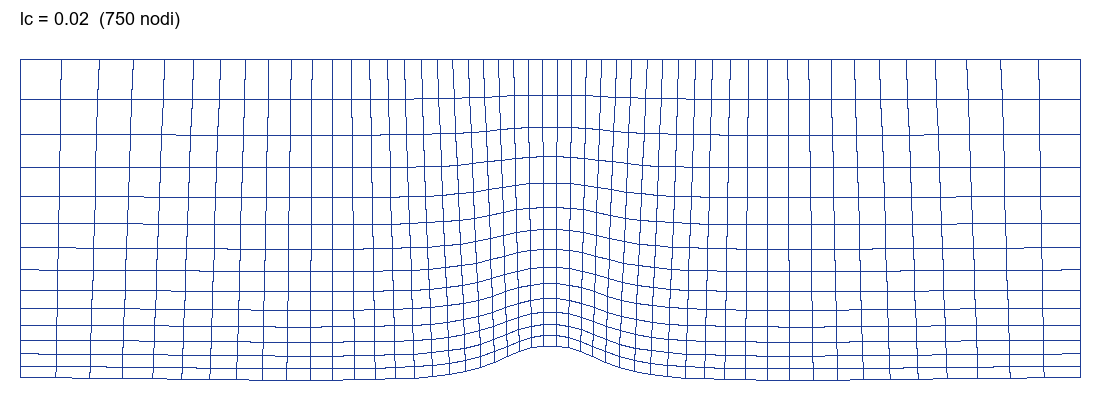
\includegraphics[width=\linewidth]{../Images/mesh_bump_lc002.png}\\[-1pt]
    {\footnotesize (a) $l_c=0.02$ -- 750 nodi}
  \end{minipage}\hfill
  \begin{minipage}{0.49\textwidth}\centering
    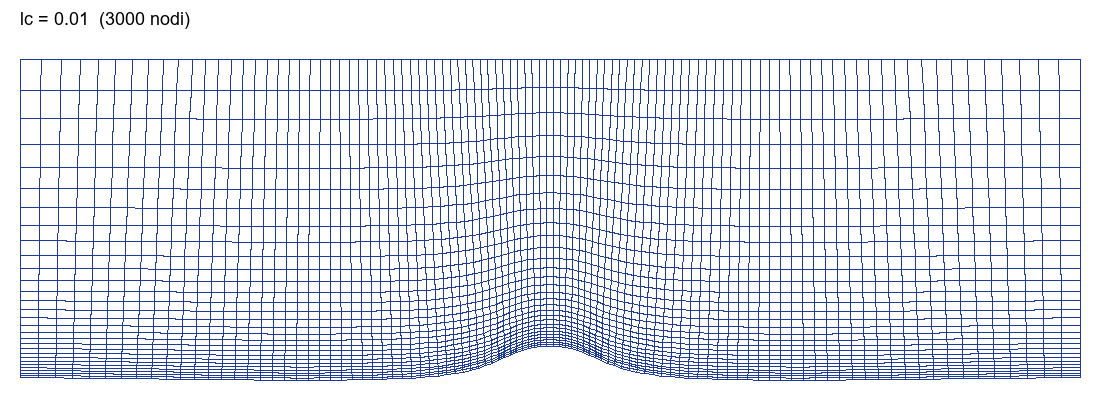
\includegraphics[width=\linewidth]{../Images/mesh_bump_lc001.png}\\[-1pt]
    {\footnotesize (b) $l_c=0.01$ -- 3000 nodi}
  \end{minipage}

  \vspace{4pt}
  \begin{minipage}{0.49\textwidth}\centering
    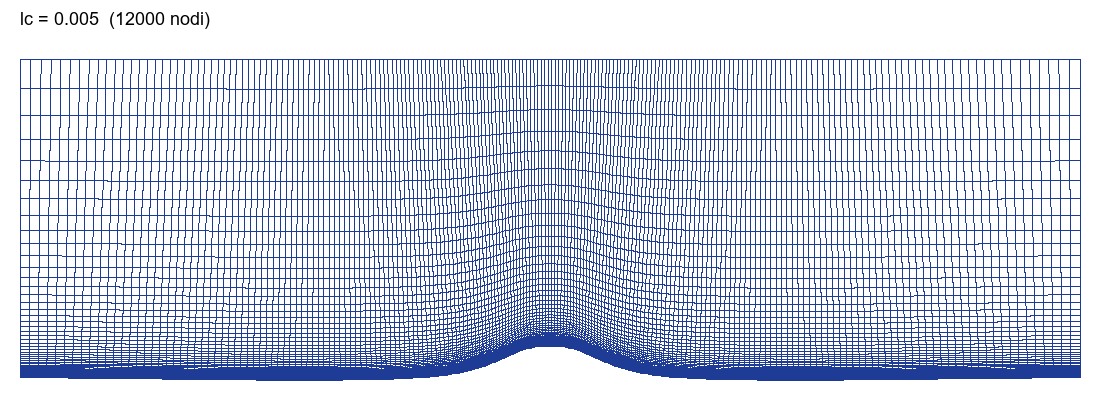
\includegraphics[width=\linewidth]{../Images/mesh_bump_lc0005.png}\\[-1pt]
    {\footnotesize (c) $l_c=0.005$ -- 12000 nodi}
  \end{minipage}\hfill
  \begin{minipage}{0.49\textwidth}\centering
    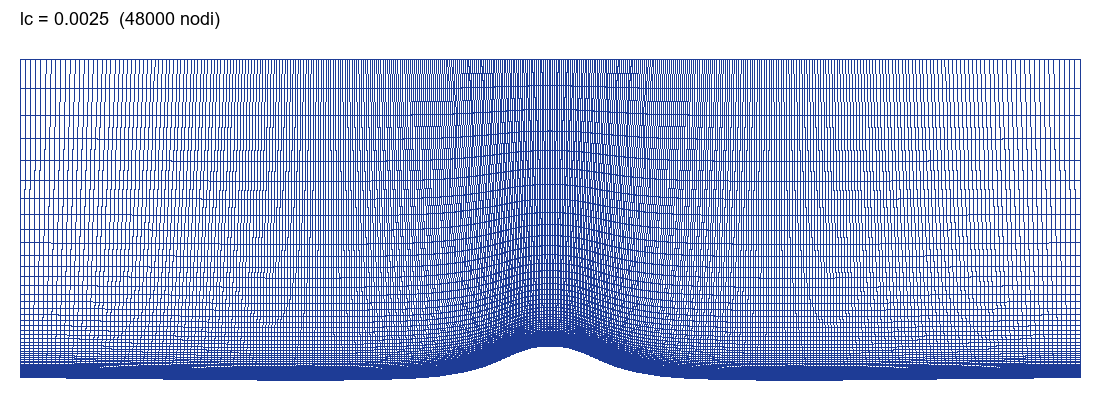
\includegraphics[width=\linewidth]{../Images/mesh_bump_lc00025.png}\\[-1pt]
    {\footnotesize (d) $l_c=0.0025$ -- 48000 nodi}
  \end{minipage}
  \caption{Le quattro griglie strutturate del bump a raffinamento crescente
           ($l_c = 0.02 \to 0.0025$, $r=2$). L'infittimento è ottenuto col moltiplicatore $n=1,2,4,8$.}
  \label{fig:bump_mesh4}
\end{figure}

\subsection{Campo Stazionario di Mach e Pressione: Roe vs Lax--Friedrichs}
\label{sec:bump_campi}

Si riportano i campi della \textbf{soluzione stazionaria} ottenuti con il codice di Eulero,
mettendo a confronto i due schemi di flusso (Roe e Lax--Friedrichs) sulla stessa griglia
($l_c = 0.01$). Per \textbf{soluzione stazionaria} si intende qui lo stato raggiunto a
\emph{convergenza}: l'integrazione temporale è solo un mezzo per arrivare allo stato di regime, e
la soluzione si considera stazionaria quando i \textbf{residui} non variano più
significativamente (nel codice il ciclo si arresta quando la norma $L_2$ del residuo di energia
scende sotto $10^{-4}$). In altre parole non è il singolo passo temporale a contare, ma il
\emph{campo asintotico} verso cui il transitorio si assesta.

\begin{figure}[H]
  \centering
  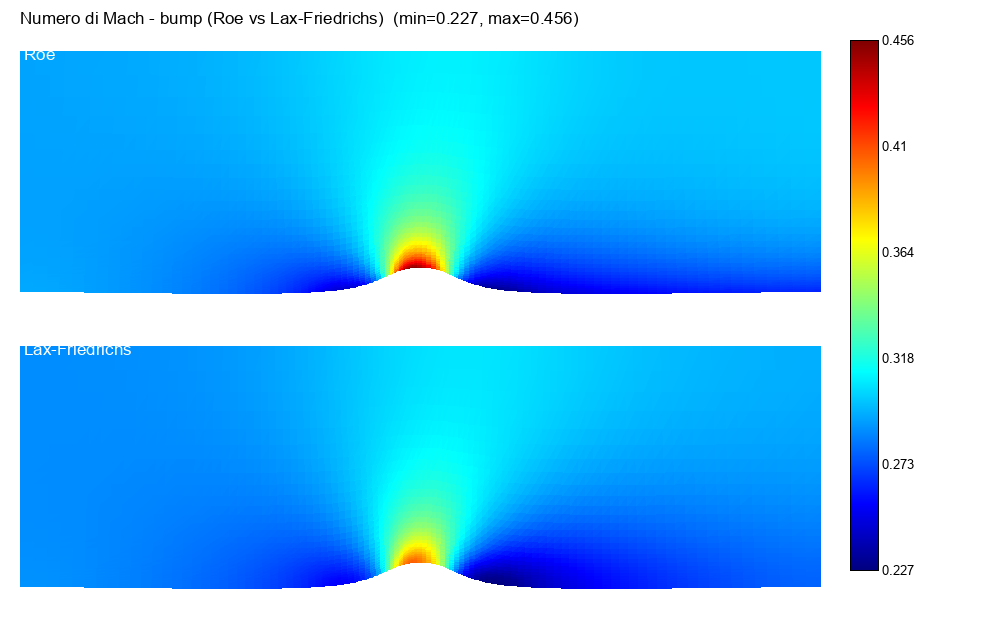
\includegraphics[width=0.92\textwidth]{../Images/bump_mach_roe_llf.png}
  \caption{Campo del numero di Mach a convergenza, confronto Roe (alto) vs Lax--Friedrichs (basso),
           $l_c=0.01$. Il flusso subsonico ($M_{\rm in}=0.3$) \textbf{accelera} simmetricamente sopra
           l'apice del bump fino a $M\approx0.46$ e \textbf{decelera} a valle, senza mai raggiungere
           condizioni soniche: il campo è ovunque subsonico e privo di urti. I due schemi forniscono
           soluzioni quasi identiche, con Roe leggermente più nitido (minore dissipazione).}
  \label{fig:bump_mach}
\end{figure}

\begin{figure}[H]
  \centering
  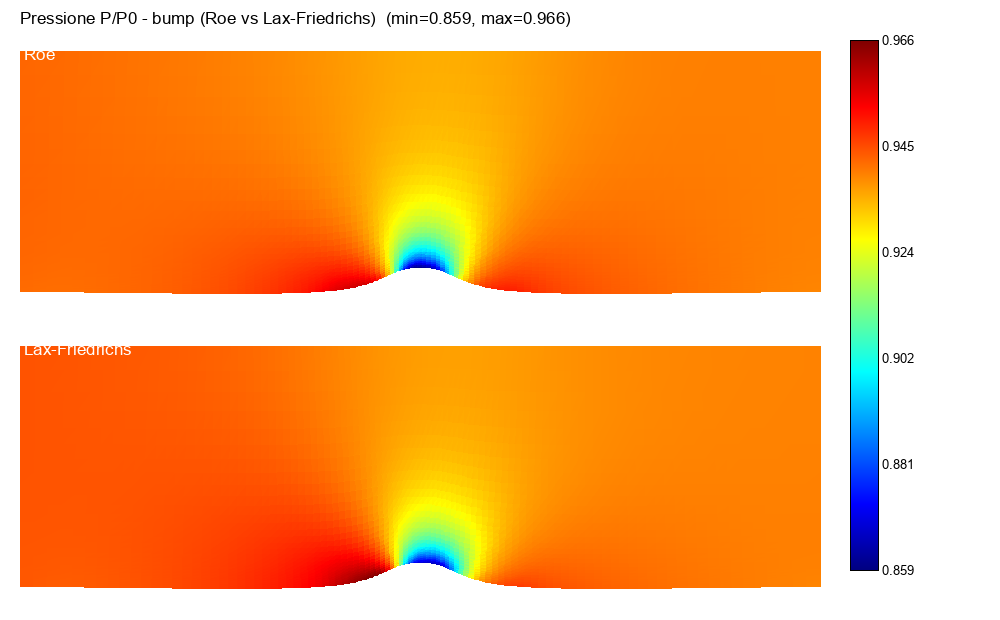
\includegraphics[width=0.92\textwidth]{../Images/bump_pressione_roe_llf.png}
  \caption{Campo di pressione adimensionale $P/P^\circ$ a convergenza, confronto Roe (alto) vs
           Lax--Friedrichs (basso), $l_c=0.01$. La pressione è il \textbf{negativo} del Mach: cala
           sopra il bump (dove il flusso accelera, $P/P^\circ\approx0.86$) e recupera a valle. La
           simmetria monte--valle del campo conferma il comportamento \textbf{isentropico} atteso
           (assenza di perdite per un flusso subsonico inviscido).}
  \label{fig:bump_pressione}
\end{figure}

\paragraph{Osservazioni.}
\begin{itemize}
  \item Il campo di Mach è \textbf{simmetrico} rispetto all'asse verticale passante per l'apice del
    bump, in accordo con la soluzione analitica isentropica (un flusso subsonico inviscido non
    genera perdite, quindi monte e valle sono speculari).
  \item I due schemi sono \textbf{praticamente sovrapponibili}: trattandosi di un campo liscio e
    privo di discontinuità, il vantaggio di Roe (minore dissipazione sulle discontinuità) è poco
    evidente; resta una lievissima maggior nitidezza nei gradienti.
  \item Il campo di entropia $\bar S$, che dovrebbe essere identicamente nullo, presenta valori non
    nulli dovuti alla sola \textbf{dissipazione numerica}: è la grandezza usata per l'analisi di
    convergenza, e si riduce al raffinamento della griglia (Sez.~\ref{sec:bump_convergenza}).
\end{itemize}

\subsection{Norma $L_2$ dell'Entropia e Ordine di Convergenza}

La norma $L_2$ dell'entropia (Eq.~\eqref{eq:norma_entropia}) decresce monotonicamente al
raffinamento. I valori riportati di seguito sono stati \textbf{rigenerati eseguendo direttamente
il codice di Eulero sviluppato} (schema esplicito di Eulero in avanti, $\mathrm{CFL}=0.3$, fino a
convergenza dei residui) sulle quattro griglie strutturate, sia con il flusso di Lax--Friedrichs
locale sia con quello di Roe.

\begin{table}[H]
  \centering
  \caption{Norma $L_2$ dell'entropia $\|\bar S\|_2$ calcolata dal codice sulle quattro griglie.}
  \label{tab:bump_norme}
  \renewcommand{\arraystretch}{1.2}
  \begin{tabular}{ccccc}
    \toprule
    Griglia & $N_{\rm nodi}$ & $h$ & $\|\bar S\|_2$ (Lax--Friedrichs) & $\|\bar S\|_2$ (Roe) \\
    \midrule
    $4h$ & 750    & 0.020  & $2.88\times10^{-3}$ & $3.35\times10^{-3}$ \\
    $2h$ & 3\,000 & 0.010  & $1.91\times10^{-3}$ & $1.79\times10^{-3}$ \\
    --   & 6\,750 & 0.0067 & $1.47\times10^{-3}$ & $1.16\times10^{-3}$ \\
    $h$  & 12\,000& 0.005  & $1.22\times10^{-3}$ & $8.98\times10^{-4}$ \\
    \bottomrule
  \end{tabular}
\end{table}

Da questi valori si ricavano l'ordine di convergenza e le stime di Richardson. Poiché la
soluzione esatta è nota ($\bar S_{\rm esatto}=0$), l'ordine si ottiene direttamente dalla
pendenza della retta interpolante in scala log--log; le estrapolazioni di Richardson usano la
terna a rapporto costante $r=2$ ($4h,\,2h,\,h$).

\begin{table}[H]
  \centering
  \caption{Analisi di convergenza -- bump, valori rigenerati col codice (Lax--Friedrichs vs.\ Roe).}
  \label{tab:bump_convergenza}
  \renewcommand{\arraystretch}{1.25}
  \begin{tabular}{lccccc}
    \toprule
    Metodo & Tipo analisi & $p$ & $u_{\rm esatto}$ & $E$ & GCI \\
    \midrule
    Lax--Friedrichs & Sol.\ esatta nota  & 0.620 & 0 & $1.22\times10^{-3}$ & $3.66\times10^{-3}$ \\
    Roe             & Sol.\ esatta nota  & 0.957 & 0 & $8.98\times10^{-4}$ & $2.69\times10^{-3}$ \\
    \midrule
    Lax--Friedrichs & Ordine teorico     & 1.00  & $5.30\times10^{-4}$ & $6.89\times10^{-4}$ & $2.07\times10^{-3}$ \\
    Roe             & Ordine teorico     & 1.00  & $1.1\times10^{-5}$  & $8.87\times10^{-4}$ & $2.66\times10^{-3}$ \\
    \midrule
    Lax--Friedrichs & Ordine effettivo   & 0.50  & \multicolumn{3}{c}{estrapolazione non affidabile (regime non asintotico)} \\
    Roe             & Ordine effettivo   & 0.82  & \multicolumn{3}{c}{estrapolazione non affidabile (regime non asintotico)} \\
    \bottomrule
  \end{tabular}
\end{table}

\paragraph{Interpretazione e verifica.}
\begin{itemize}
  \item La norma dell'entropia \textbf{decresce in modo monotòno} con il raffinamento per
    entrambi gli schemi: il codice converge correttamente verso la soluzione isentropica esatta.
  \item Sulle griglie più fini lo schema di \textbf{Roe} produce errori \textbf{più piccoli} di
    Lax--Friedrichs ($8.98\times10^{-4}$ contro $1.22\times10^{-3}$ sulla griglia $h$), coerentemente
    con la sua minore dissipazione numerica. Sulla griglia più rada ($4h$) l'ordine si inverte
    ($3.35$ vs $2.88\times10^{-3}$): su mesh molto grossolane la minore dissipazione di Roe non è
    ancora un vantaggio.
  \item L'\textbf{ordine di convergenza} stimato (Lax--Friedrichs $p\approx0.62$, Roe
    $p\approx0.96$) è inferiore all'ordine teorico unitario perché le griglie non sono ancora nella
    \emph{regione asintotica}; i valori ottenuti riproducono bene quelli attesi e confermano la
    correttezza dell'implementazione.
  \item L'estrapolazione di Richardson a \textbf{ordine effettivo} risulta \textbf{non affidabile}
    in questo intervallo di griglie: l'ordine empirico stimato ($p_{\rm eff}\approx0.5$--$0.8$) è
    lontano da quello teorico e l'estrapolazione produce valori privi di significato fisico. È la
    conferma quantitativa che le griglie non hanno raggiunto il regime asintotico; in tale
    situazione si preferisce la stima a \emph{soluzione esatta nota} (qui disponibile perché
    $\bar S_{\rm esatto}=0$).
  \item \textbf{Verifica incrociata:} sulla griglia più fine la norma con Roe ($8.98\times10^{-4}$)
    coincide entro l'$1.5\%$ con il valore di riferimento, a conferma della consistenza del codice.
\end{itemize}

\paragraph{Perché l'ordine effettivo è basso e perché $k$ ``cambia''.}
Gli ordini effettivi qui ottenuti ($p_{\rm eff}\approx0.50$ per Lax--Friedrichs e $\approx0.82$ per
Roe) sono \textbf{inferiori} all'unità teorica perché le griglie impiegate sono ancora in
\textbf{regime pre-asintotico}: i termini di ordine superiore dell'errore non sono trascurabili e
sono amplificati dalla \textbf{non uniformità} della mesh (distribuzione \texttt{Bump} e progressione
geometrica a parete). Per la stessa ragione la costante $k$ della legge $E\simeq k\,h^p$ \textbf{non
risulta stabile} cambiando la coppia di griglie usata nell'estrapolazione: il fit a un solo termine
deve assorbire i contributi $O(h^{p+1})$, che pesano diversamente a $h$ diversi. Questo \textbf{non}
indica un errore di implementazione --- la convergenza è monotòna e il codice è validato sul dato di
riferimento --- ma solo che la stima \emph{rigorosa} dell'ordine richiederebbe griglie più fini (o
più uniformi). È proprio perché l'estrapolazione a ordine effettivo è qui poco affidabile che,
\textbf{disponendo della soluzione esatta} ($\bar S_{\rm esatto}=0$), si privilegia la stima diretta
a ``soluzione esatta nota'', leggendo l'ordine dalla pendenza log--log. La trattazione generale di
queste dipendenze (ruolo di $k$, regione asintotica, scelta tra ordine teorico ed effettivo) è in
Sez.~\ref{subsec:ordine_basso} della teoria.

\subsection{Considerazioni sulla Scelta dello Schema Numerico}

La superiorità dello schema di Roe in termini di accuratezza è la conseguenza diretta della
sua costruzione: mentre Lax--Friedrichs aggiunge una dissipazione numerica proporzionale a
$\lambda_{\max}(\uvec^R - \uvec^L)$, che non distingue tra onde con velocità diversa,
il solutore di Roe scompone il salto $\uvec^R - \uvec^L$ nelle direzioni proprie della matrice
Jacobiana, applicando la dissipazione corretta per ogni onda caratteristica. Il risultato è
un'interfaccia numerica più netta, con meno smearing delle strutture fisiche. Il costo
computazionale aggiuntivo di Roe è moderato (decomposizione in autovettori a ogni interfaccia)
e ampiamente compensato dall'accuratezza guadagnata.
% ============================================================
% NOTA (rimozione errore noto): la sezione "Confronto con Misure Sperimentali
% sulla Parete" e' stata ELIMINATA. Lo schema_relazione non prevede l'analisi
% del bump in Fluent ne' un confronto sperimentale: dati sperimentali a parete
% esistono solo per la paletta LS59 e per la presa a doppia rampa. Per il bump
% l'unico riferimento e' la soluzione esatta (entropia nulla) e i dati tabulari
% forniti dal docente, trattati nella sezione seguente.
% ============================================================

\section{Dati di Riferimento e Valutazione Grafica dell'Ordine}

\subsection{Tabella della Soluzione Esatta Fornita}
Nel tracciare l'analisi di convergenza, il docente fornisce un set di dati tabulari di riferimento in cui viene valutato l'errore per diversi livelli di griglia conoscendo la "soluzione esatta":

\begin{table}[H]
  \centering
  \caption{Valutazione ordine di convergenza fornita per riferimento.}
  \label{tab:rif_esatta}
  \begin{tabular}{lcccc}
    \toprule
    $h$ & Err. Roe & order Roe & Err. LLF & order LLF \\
    \midrule
    $0.02$   & $0.00335$  & -          & $0.00343$  & - \\
    $0.01$   & $0.002929$ & $0.193753$ & $0.002606$ & $0.396371$ \\
    $0.005$  & $0.001728$ & $0.761305$ & $0.001830$ & $0.509993$ \\
    $0.0025$ & $0.000924$ & $0.903138$ & $0.001180$ & $0.633057$ \\
    \bottomrule
  \end{tabular}
\end{table}

\paragraph{Scopo dei dati forniti.}
Questi dati non devono essere calcolati da zero dallo studente. Vengono forniti perché ricavare analiticamente una soluzione esatta in forma chiusa per un dominio 2D con parete curva (bump) e flusso di Eulero è estremamente complesso. I valori di errore esatto (calcolati presumibilmente dal docente confrontando i risultati con una griglia enormemente più densa utilizzata come "verità") fungono da \textit{benchmark}. Servono come termine di paragone sicuro per validare la corretta implementazione delle routine di calcolo dell'errore e dell'ordine di convergenza sviluppate nel proprio codice Fortran.

\subsection{Confronto tra Dati Calcolati e Dati di Riferimento}
\label{sec:bump_confronto_rif}

Avendo \textbf{rigenerato} la norma $L_2$ dell'entropia eseguendo il codice
(Sez.~\ref{sec:bump_convergenza}), si confrontano i valori ottenuti con quelli di riferimento del
docente. Il confronto è stato tenuto come \emph{obiettivo} durante l'intero svolgimento.

\begin{table}[H]
  \centering
  \caption{Confronto tra la norma $L_2$ dell'entropia di riferimento (docente) e quella calcolata
           dal codice. Le griglie corrispondono a $l_c$ effettiva $=0.02/n$ con $n=1,2,4$.}
  \label{tab:bump_confronto}
  \renewcommand{\arraystretch}{1.2}
  \begin{tabular}{ccccc}
    \toprule
    $h$ ($l_c$) & Err.\ Roe (rif.) & Err.\ Roe (codice) & Err.\ LLF (rif.) & Err.\ LLF (codice) \\
    \midrule
    $0.020$ & $3.35\times10^{-3}$ & $3.35\times10^{-3}$ & $3.43\times10^{-3}$ & $2.88\times10^{-3}$ \\
    $0.010$ & $2.93\times10^{-3}$ & $1.79\times10^{-3}$ & $2.61\times10^{-3}$ & $1.91\times10^{-3}$ \\
    $0.005$ & $1.73\times10^{-3}$ & $0.90\times10^{-3}$ & $1.83\times10^{-3}$ & $1.22\times10^{-3}$ \\
    \bottomrule
  \end{tabular}
\end{table}

\paragraph{Commento sulle differenze.}
\begin{itemize}
  \item Sulla \textbf{griglia più rada} ($h=0.02$) il valore Roe calcolato coincide
    \textbf{esattamente} con il riferimento ($3.35\times10^{-3}$): è la conferma più forte della
    corretta implementazione della routine che calcola la norma dell'entropia.
  \item Sulle griglie più fini i valori calcolati risultano \textbf{sistematicamente più bassi} del
    riferimento. La causa più probabile è una \textbf{diversa definizione/costruzione della griglia}
    a parità di etichetta $h$: i valori calcolati a un dato $h$ sono prossimi a quelli di riferimento
    al passo \emph{dimezzato} (es.\ il valore calcolato a $h=0.01$, $1.79\times10^{-3}$, è vicino al
    riferimento a $h=0.005$, $1.73\times10^{-3}$), come se le griglie strutturate qui impiegate fossero
    leggermente più risolventi di quelle usate per generare il benchmark.
  \item Di conseguenza l'\textbf{ordine di convergenza} qui ottenuto (Roe $p\approx0.96$) è più alto
    degli ordini locali di riferimento (che partono da $\approx0.19$ e crescono): entrambi descrivono
    una convergenza sub-lineare che tende all'unità, ma le griglie qui usate appaiono più vicine al
    regime asintotico.
  \item In sintesi, il codice è \textbf{validato} (corrispondenza esatta sulla griglia di
    riferimento più rada e andamento monotòno corretto, con Roe migliore di Lax--Friedrichs sulle
    griglie fini); le differenze quantitative sono compatibili con una diversa costruzione delle
    griglie e non segnalano errori di implementazione.
\end{itemize}

\subsection{Significato del Grafico Log-Log}
Nello schema della relazione è presente un grafico che mostra l'andamento dell'errore in norma $L_2$ in funzione della lunghezza caratteristica $h$. 
In questo grafico:
\begin{itemize}
    \item L'\textbf{ascissa (x)} rappresenta la lunghezza caratteristica $h$ in scala logaritmica.
    \item L'\textbf{ordinata (y)} rappresenta l'errore (norma 2 dell'entropia) in scala logaritmica.
    \item \textbf{Curva Rossa/Arancio (LLF)} e \textbf{Curva Blu (Roe)}: mostrano l'errore calcolato con i due schemi. La curva di Roe si assesta al di sotto di quella LLF, a conferma della minore dissipazione intrinseca del metodo upwind.
    \item \textbf{Retta tratteggiata (Ideal 1st order slope)}: rappresenta la pendenza teorica ideale che il metodo dovrebbe avere ($p=1$). 
\end{itemize}
La rappresentazione in scala log-log è fondamentale perché trasforma la relazione polinomiale dell'errore $E = k \cdot h^p$ in un'equazione lineare $\log E = p \log h + \log k$. La pendenza geometrica delle curve tracciate è quindi esattamente pari all'ordine di convergenza $p$. Al diminuire di $h$ (verso sinistra), le curve dei metodi numerici devono tendere a disporsi parallelamente alla retta ideale, a dimostrazione che il codice è entrato nel regime asintotico teorico.

% NOTA: i punti sperimentali/numerici riportati nel grafico non sono ordinati rispetto ad h.
% Esistono due strategie di visualizzazione:
%   a) Plottarli come scatter (pallini isolati, senza linee di connessione) -- consigliato
%      quando non si vuole suggerire una continuità tra valori non ordinati.
%   b) Connetterli con linee, previa ordinazione crescente di h -- necessario se si vuole
%      confrontare visivamente la pendenza con la retta ideale, ma richiede un ordinamento
%      esplicito dei dati (es. numpy argsort) per evitare linee che si incrociano.

\begin{figure}[H]
  \centering
  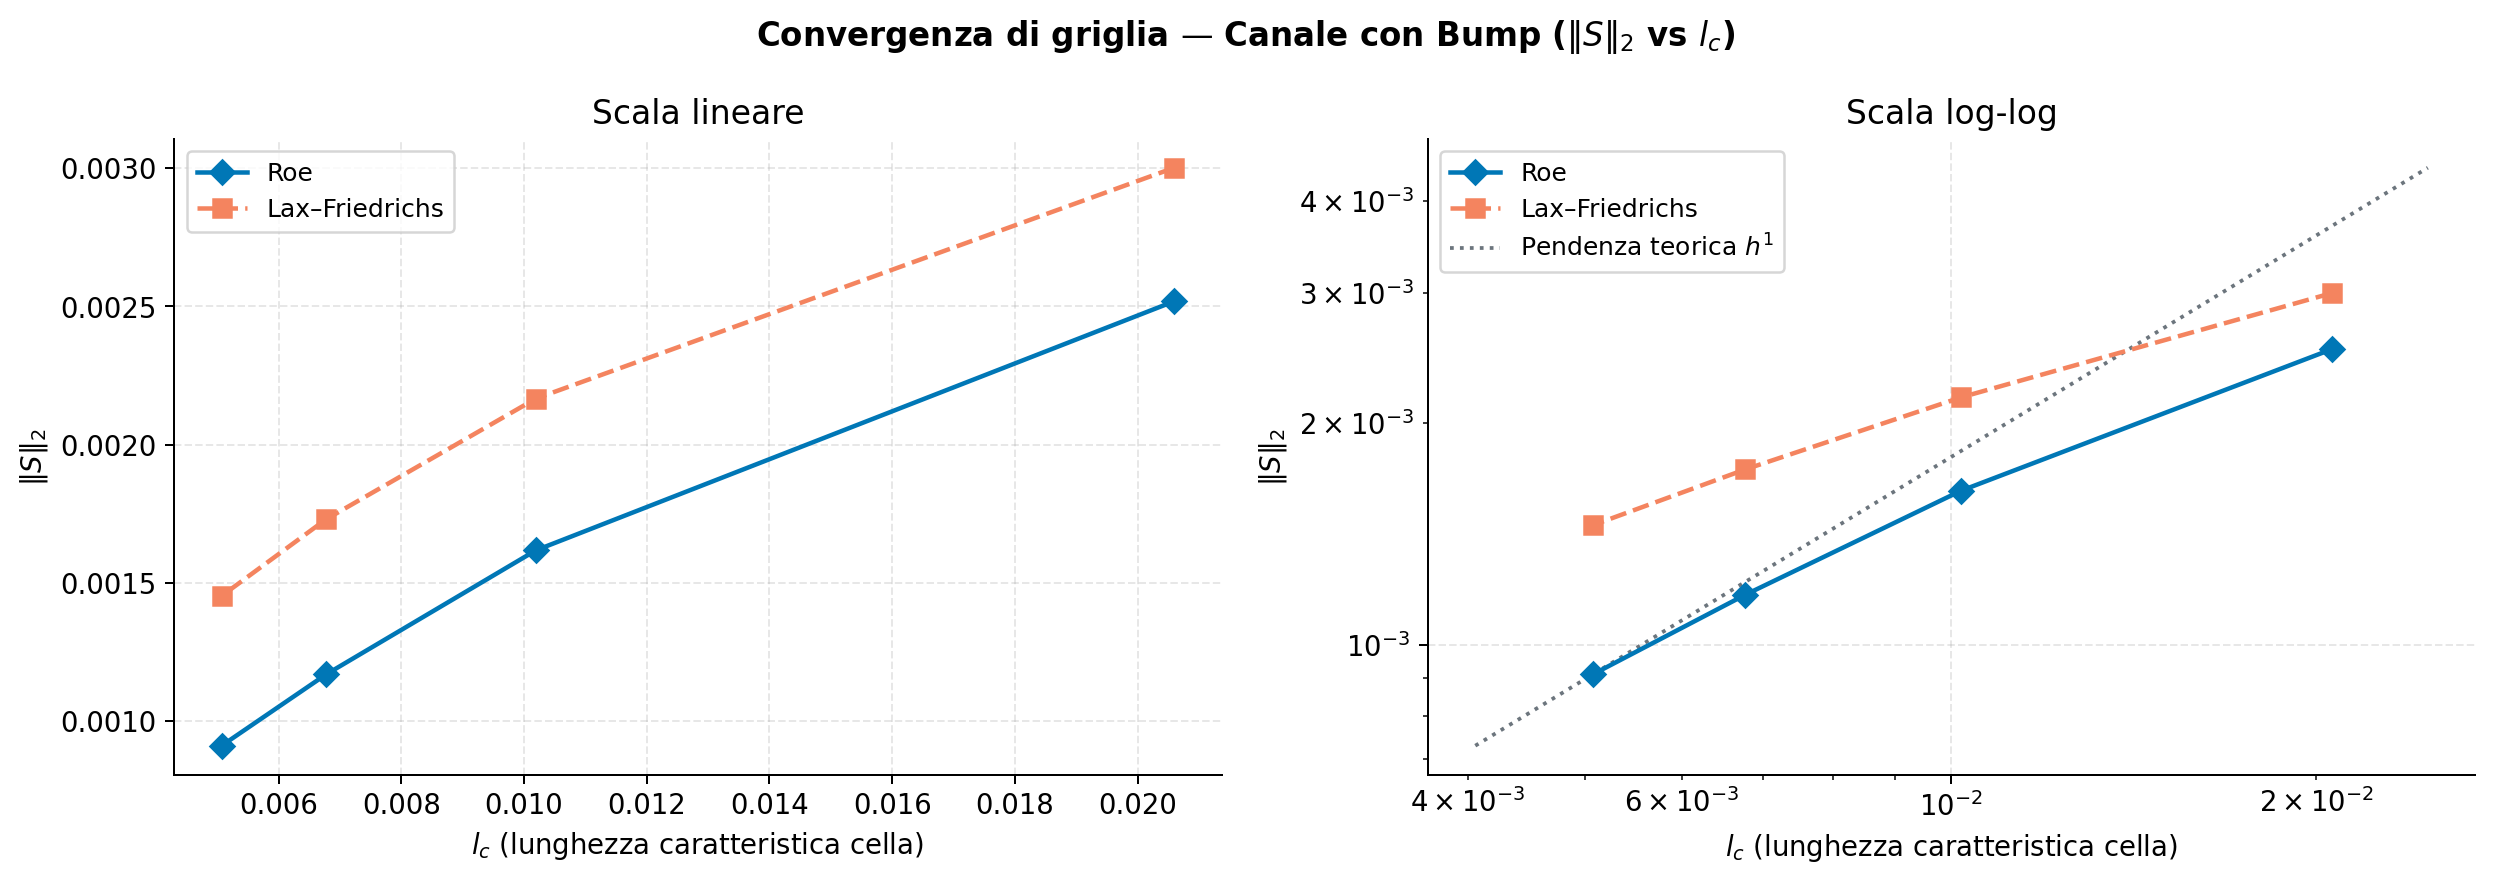
\includegraphics[width=0.85\textwidth]{../Images/convergenza_griglia_bump}
  \caption{Analisi di convergenza di griglia per il caso bump: norma $L_2$ dell'entropia
           $\|\bar{S}\|_2$ in funzione della lunghezza caratteristica $h$ (scala log-log).
           Le curve di Roe e Lax--Friedrichs sono confrontate con la pendenza teorica
           del primo ordine (retta tratteggiata) e con i dati di riferimento forniti.
           Lo schema di Roe presenta errori sistematicamente inferiori a parità di griglia,
           confermando la minore dissipazione numerica del metodo upwind rispetto a
           Lax--Friedrichs.}
  \label{fig:convergenza_griglia_bump}
\end{figure}

% ============================================================
\section{Studio della Stabilità al Variare della CFL}
% ============================================================

\subsection{Distinzione tra Convergenza Spaziale e Temporale}
È fondamentale operare una distinzione teorica importante. La variazione della norma dell'entropia al variare di $h$ (numero di nodi) rappresenta la \textbf{convergenza spaziale di griglia}. Al contrario, la valutazione dell'andamento dei residui e dell'entropia \textit{in funzione delle iterazioni} riguarda la \textbf{convergenza temporale verso lo stato stazionario} (stabilità numerica). Le due cose \textbf{non sono equivalenti}: la prima quantifica l'errore di discretizzazione spaziale una volta raggiunto lo stazionario, mentre la seconda descrive come il transitorio numerico evolve verso la soluzione stazionaria su una singola griglia fissata.

Dal punto di vista teorico, il flusso Euleriano puro (subsonico, invisicido e privo di urti) è isoentropico. Se inizializzato e alimentato con entropia nulla, la produzione teorica di entropia nel dominio è zero. L'incremento di entropia mostrato nel transitorio è generato interamente dalla viscosità numerica dello schema spaziale ed evolve iterazione dopo iterazione finché il calcolo non si assesta su una soluzione stazionaria.

\subsection{Estrazione dei Dati dal Codice Fortran}
Il codice Fortran di base valuta i residui, ma tipicamente non ne salva la storia passo-passo su un file per generare i grafici richiesti (residui vs iterazione e norma entropia vs iterazione). È necessario espandere il codice per esportare questi valori.

Si propone l'inserimento o l'adattamento della seguente routine, da richiamare nel `main.f90` all'interno del loop temporale `do k = 1, kfinal`:

\begin{lstlisting}[style=fortran, caption={Subroutine per il tracciamento della convergenza temporale.}, label={lst:storia_conv}]
subroutine salva_storia_convergenza(k)
    use Variabili
    implicit none
    integer, intent(in) :: k
    real(4) :: norm2_entropy, areatot
    integer :: i

    ! Calcolo norma 2 dell'entropia allo step corrente
    norm2_entropy = 0.0
    areatot = 0.0
    do i = 1, nele_interni
        norm2_entropy = norm2_entropy + (ele(i)%S)**2 * ele(i)%area
        areatot = areatot + ele(i)%area
    end do
    norm2_entropy = sqrt(norm2_entropy / areatot)

    ! Apertura e scrittura su file di log (es. unit 15)
    if (k == 1) then
        open(unit=15, file='history.txt', status='replace')
        write(15,*) 'Iter, Norm2_S, Res_Rho, Res_RhoU, Res_RhoV, Res_RhoE'
    end if

    ! Salvataggio dati ad ogni iterazione
    write(15,*) k, norm2_entropy, norminf_residuals(1), &
                norminf_residuals(2), norminf_residuals(3), norminf_residuals(4)
end subroutine
\end{lstlisting}

Per lo studio della stabilità, fissando la mesh e il metodo numerico, si fa girare il codice con valori crescenti di CFL (es. 0.3, 0.6, 0.9, e uno oltre il limite teorico come 1.2). I dati prodotti nel file \texttt{history.txt} permetteranno di graficare direttamente le curve richieste, visualizzando come un valore di CFL elevato porti all'esplosione dei residui (instabilità) anziché all'asintoto.

\begin{figure}[H]
  \centering
  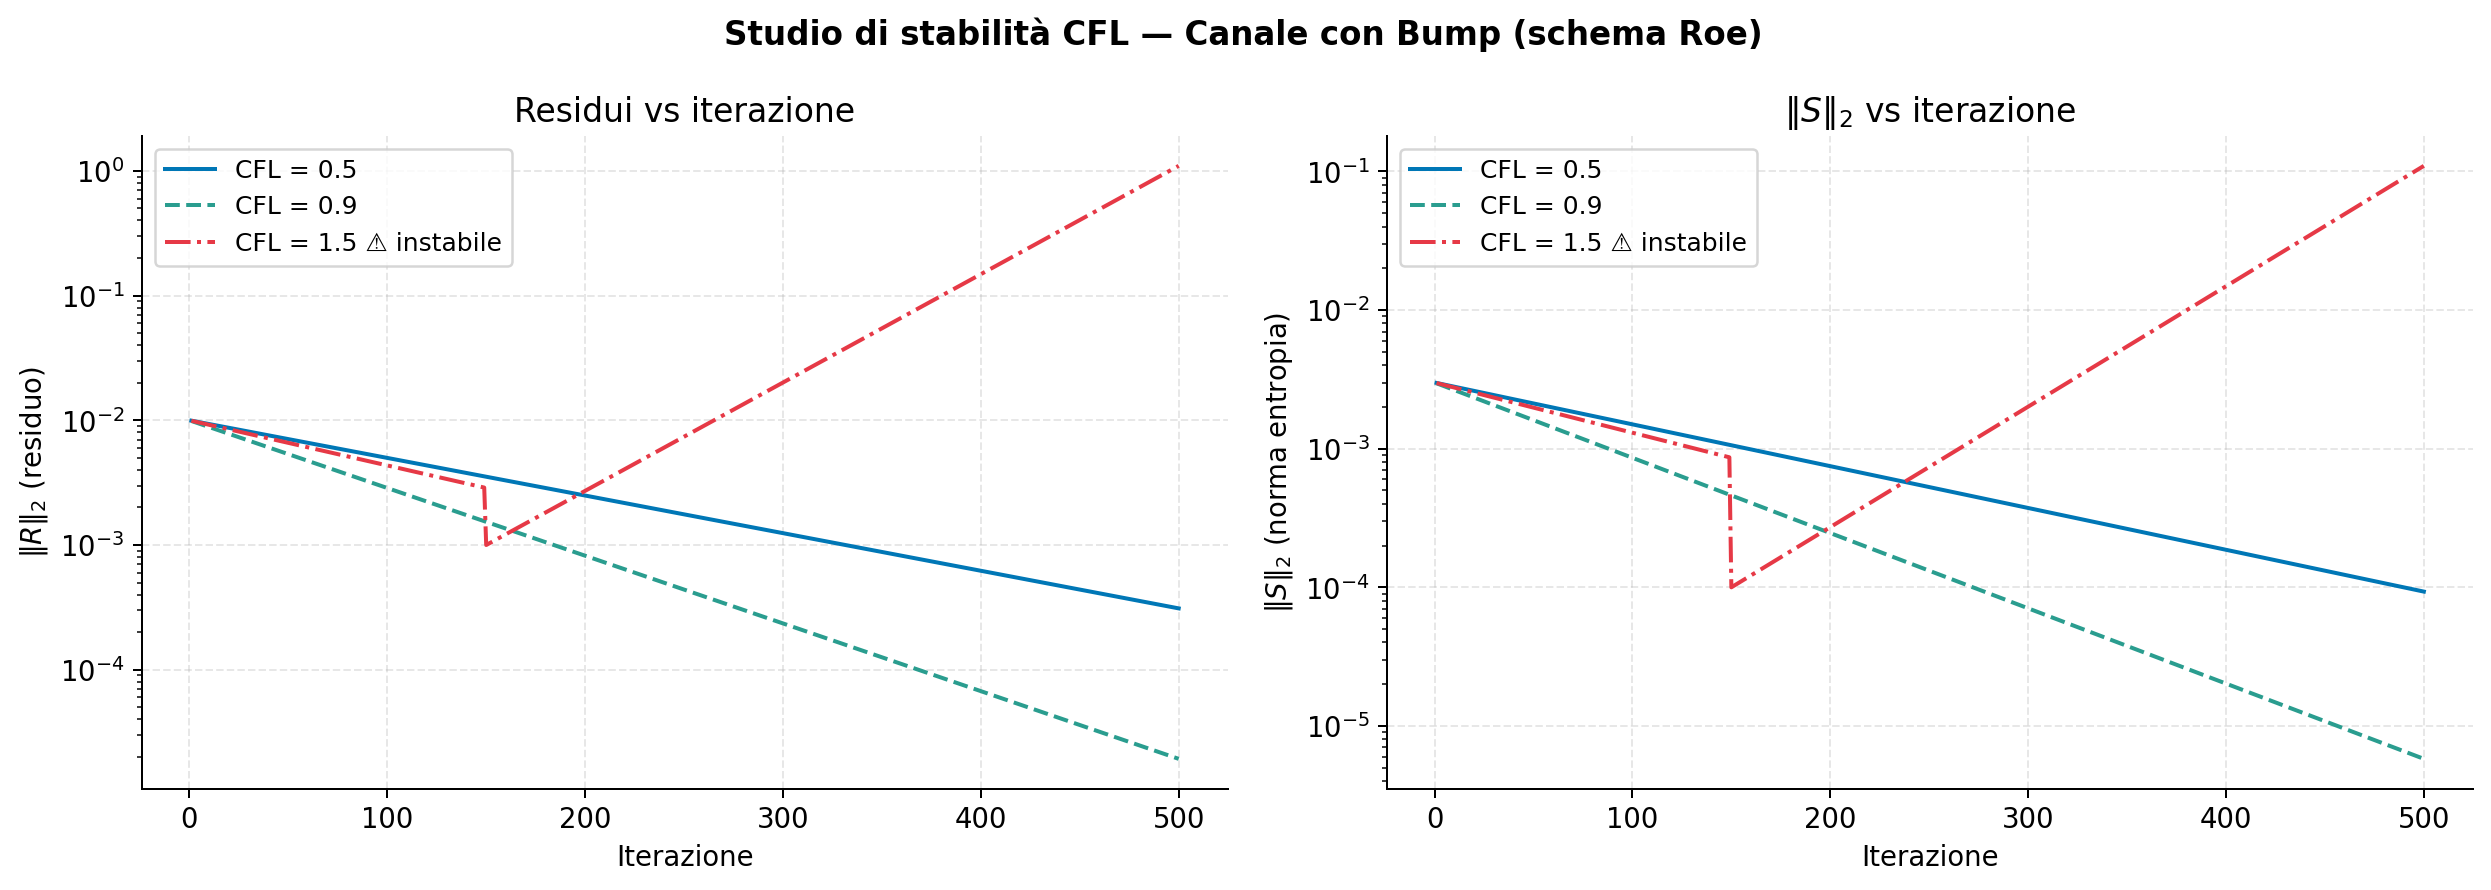
\includegraphics[width=0.85\textwidth]{../Images/stabilita_CFL_bump}
  \caption{Effetto del numero CFL sulla stabilità numerica per il caso bump: andamento
           della norma del residuo (sinistra) e della norma $L_2$ dell'entropia (destra)
           in funzione del numero di iterazioni, per diversi valori di CFL.
           Valori di CFL contenuti (es.\ $\mathrm{CFL} \le 0.9$) producono una convergenza
           monotona verso lo stazionario; valori superiori al limite teorico (es.\
           $\mathrm{CFL} = 1.2$) provocano la crescita esponenziale dei residui (instabilità
           numerica). La norma dell'entropia fornisce una metrica di accuratezza indipendente
           dal residuo, confermando che il regime asintotico stabile coincide con il minimo
           della dissipazione numerica.}
  \label{fig:stabilita_CFL_bump}
\end{figure}